\section{Problem Statement}
\label{sec:problem}
%
Alice has a $5 \times 5$ chess board as shown in Figure~\ref{fig:problem}, where
each square is described by its coordinates $(i, j) \in \{0, 1, 2, 3, 4\}^2$.
Her remote-controlled robot starts on the square $(2,2)$. The remote-controller
has $4$ buttons that can move the robot east, north, west, and south by 1 square
with each press. Bob, her mischievous sibling, has tampered with the wiring of
these buttons. Assuming that the buttons are fixed after having shuffled once,
what is the expected value of the minimum number of times Alice needs to press
the buttons in order to move the robot to the goal square $(4,4)$?

\begin{figure}[bth]
    \centering
    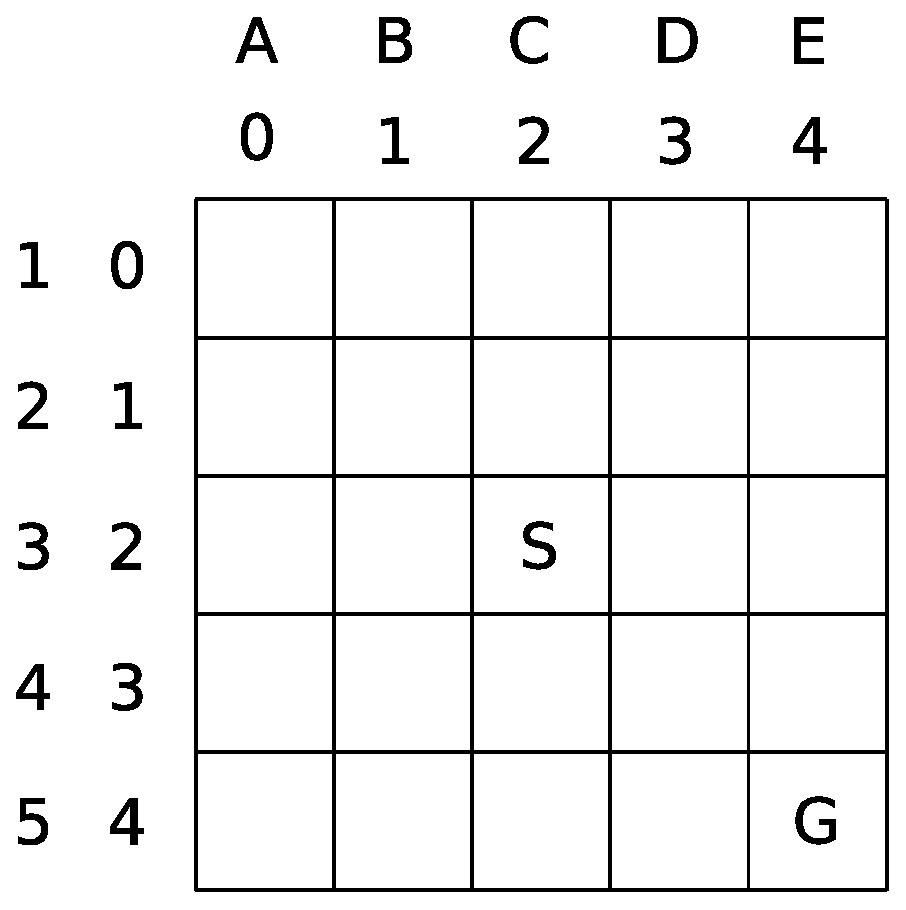
\includegraphics[width=0.25\textwidth]{./figures/drawing_v1.eps}
    \caption{Schematic of the problem.}
    \label{fig:problem}
\end{figure}
%
In this setup, we assume that the agent has knowledge of the environment it is
in; i.e., the agent knows the map of the environment. This means, in particular,
that the agent would know that it needs to try a different key whenever it 
reaches the boundary of the chessboard by hitting (since hitting this key
obviously would try and move the robot into the wall, wasting a key press).

A second observation to be made is that the agent should not make any more
than $2$ mistakes because once $2$ mistakes are made, the remaining actions 
would make progress towards the goal and the agent has time to register the 
fact that it is making progress. Hence, the worst-case scenario is that the 
agent takes $8$ steps to solve the environment. Of course, it may get lucky and 
stumble upon the right combination of motions (``right'' and ``down'') in the 
first two tries, reaching the goal position in $4$ steps; however, this is not 
guaranteed.

If we linearly index the squares of the chessboard from $0$ to $24$ in a
row-major fashion, then the mapping from the linear index to the $(i, j)$
coordinates and back is given by the following bijections:
%
\begin{equation}
5j + i = k \leftrightarrow \left(i = k - 5 \floor*{\frac{k}{5}}, j = \floor*{\frac{k}{5}}\right) 
\label{eq:bijection}
\end{equation}
%
This mapping is useful and relevant for implementing the $Q$-learning algorithm
for the RL solution to the problem.